\documentclass{beamer}

\usepackage{svg}

\usetheme{Boadilla}

% Title
\title{Introduction to the Linux Shell}
\subtitle{Linux Week \the\year{}}
\author{Soham S Gumaste}
\date{\today}
\institute{Linux Users Group @ UIC}

\begin{document}
\begin{frame}
	\titlepage
\end{frame}

\begin{frame}{What is a shell?}
	A \texttt{shell} is the outermost layer of the operating system. Hence,
	a "shell"!
\end{frame}

\begin{frame}{Okay but what does that mean?}
	Modern operating systems offer a plethora of features that we take for
	granted these days.
	
	\pause

	\begin{exampleblock}{Example}
		Running multiple processes, Process Isolation, Scheduling (Take
		CS 461 to learn more!)
	\end{exampleblock}

	\pause

	Shells like \texttt{bash} expose these features in a manageable way!
\end{frame}

\begin{frame}{Shell Feature: Run a program}
	\begin{figure}
		\centering
		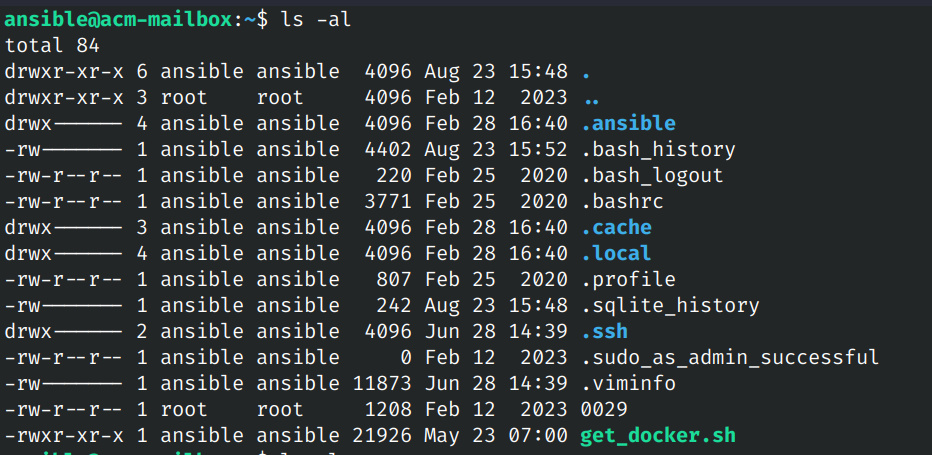
\includegraphics[width=\textwidth]{example.png}
	\end{figure}
\end{frame}

\begin{frame}{Shell Feature: Run a program}
	In this example, the shell (in this case \texttt{bash}) does the
	following:
	\pause
	\begin{itemize}
		\item Find the program named \texttt{ls} (uses the PATH variable)
			\pause
		\item If the program is found, tell the OS to load the program
			to memory and to start running it immediately.
			\pause
		\item Make sure the \texttt{ls} program gets the arguments
			specified.
	\end{itemize}
\end{frame}

\begin{frame}{Shell Feature: Store output for later}
	The shell lets you store the output of \textbf{any} command to a file
	for future use!

	\begin{block}{Syntax}
		\texttt{command > filename}
	\end{block}
\end{frame}

\begin{frame}{Shell Feature: Connect output to input!}
	This is one of the most powerful features the shell offers!

	Consider this example: I have a file with a LOT of information, and I
	want to find the number of lines in the file.
	
	\pause

	\begin{block}{Solution}
		\texttt{cat filename | wc -l} Where:
		\begin{itemize}
			\item \texttt{cat} is a command that just prints out
				the file The \texttt{|} character
				\textbf{pipes} the output of \texttt{cat} to
				the input of \texttt{wc}
			\item \texttt{wc} is a command that does
				\underline{W}ord \underline{C}ounts, but with
				the \texttt{-l} option, does line counts!
		\end{itemize}
	\end{block}
\end{frame}

\begin{frame}{The possibilities are ENDLESS!}
	There is no limit on how many commands you can chain together.

	Stay tuned to LUG@UIC for more on this topic!
\end{frame}

\begin{frame}{Closing Remarks}
	\begin{center}
		\Huge Thank you!
	\end{center}
\end{frame}

\begin{frame}{Closing Remarks}
	\begin{columns}
		\begin{column}{0.5\textwidth}
			\textbf{Officers}
			\begin{figure}
				\centering
				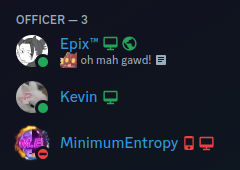
\includegraphics[width=0.60\textwidth]{officers.png}
			\end{figure}
		\end{column}
		\begin{column}{0.5\textwidth}
			The information in this presentation will be made
			available\footnotemark on our website!\\
			\url{https://lug.cs.uic.edu}
			
			\bigskip
			Join our Discord!

			\begin{figure}
				\centering
				\includesvg[width=0.5\textwidth]{lug-discord.svg}
				\caption{\url{https://discord.gg/NgxTR7PX5e}}
			\end{figure}
		\end{column}
	\end{columns}

	\footnotetext{sooner or later}
\end{frame}

\end{document}

% vim: set tw=80 ts=4 sw
